\chapter{Debugging Long Infection Chains with Interactive Dynamic Slicing}

% context
Improvements in manual debugging, such as back-in-time debugging, allow developers to debug a program more efficiently in general, but do not assist developers in finding code related to a specific problem.
\Ac{afl} techniques, such as spectrum-based fault analysis or slicing \todo{cite}, can help developers to locate faults by suggesting relevant code locations.
However, developers still need to manually debug the code to identify erroneous state at the suggested locations.
Furthermore, many \ac{afl} tools generate a lot of knowledge about a program's execution in order to find the most helpful suggestions, but then discard this knowledge after the result has been produced.
Not only are developers left with no explanation why a certain code location was considered relevant, but there is also no way to search the vast body of knowledge for helpful insights.

% problem
In large and complex applications, the length of the infection chain, i.e., the distance between the code location of the observed failure and the actually defective code, can be very long.
This reduces the effectiveness of \ac{afl} approaches and makes manual debugging more tedious and time-consuming.
With growing program size, \ac{afl} approaches also often become relatively slow.
While it still may be feasible for developers to run AFL tools to gain initial suggestions on where to start a debug session, the expected waiting time can discourage the use of \ac{afl} tools during debugging.

% contribution
To better help developers debugging long infection chains, we propose to combine automated and manual debugging techniques in a single debugging tool. 
By combining the benefits of both approaches, we expect a synergy that allows for more effective debugging of long infection chains than with two independent tools.

In our work, we combined back-in-time debugging with dynamic slicing.
Our contributions in this field are threefold:
\begin{itemize}
	\item A new configurable slicing algorithm allows quick and iterative refinement of the slicing criteria to adapt the slice to changing developer questions.
	Developers can formulate their question by choosing from different dependency types that will change the outcome of the slice.
	\item The \emph{Slice Navigator} is a UI component that bundles access to the debugger and the slicer.
		It provides context for the current instruction by showing relevant parts of the slice, allows developers to iteratively refine the slicing criteria, and serves as an alternative to breakpoints and stepping.
	\item The integration of dynamic analyses directly in the debugger not only reduces interruptions in developer flow by minimizing context switches between tools and shortens waiting time as recorded run-time data can be re-used; it also allows for a new debugging workflow where developers can isolate a bug by iteratively slicing away correct code.
\end{itemize}
Furthermore, we conducted a user study that suggests less time is needed to follow an infection chain with the Slice Navigator than with traditional or back-in-time debuggers.

\section{Better Slices with Iterative Criteria Refinement}

\todo{opening paragraph}

\subsection{The Evolution of Slicing Algorithms}

In 1981, Weiser introduced slicing as a technique helping developers to find related code for a given question~\cite{weiser_81_program_slicing}.
According to Weiser, a slice is a subset of a program that, when executed, yields the same state trajectory with respect to given slicing criteria that the original program would.
The slicing criteria are pairs of variables and code locations.
An important property of the resulting slice is that it must be executable.
This allows the slice to be compiled and inspected with a debugger.

Weiser proposed an algorithm for computing static slices, i.e., slice that are correct for every possible input of the program.
Static slices often are very large, especially for complex applications, and many sophisticated methods have been developed to reduce the size of static slices \todo{ref}.

In 1990, Korel and Laski proposed to compute slices that are valid only for one specific program input~\cite{korel_88_dynamic_program_slicing}.
Such dynamic slices can be much smaller than static slices because the slicer has to consider only one concrete execution path~\cite{venkatesh_95_experimental_results_from_dynamica, hoffner_95_evaluation_and_comparison}.
However, to achieve this we must add the program input to the slicing algorithm's parameters.

Shortly after Korel and Laski, Agrawal and Horgan independently also introduced dynamic slices~\cite{agrawal_90_dynamic_program_slicing}.
Agrawal and Horgan used an approach based on execution traces that allowed to remove more statements than previous approaches, but the resulting slices were not always executable.
Thus, they defined "accurate slices" as slices that contain all statements relevant for computing the state trajectory for the slicing criteria, but are not necessarily executable.
Agrawal \etal\ also presented SPYDER, a tool that allows debugging non-executable slices by superimposing the slice on an execution of the full program~\cite{agrawal_93_debugging_with_dynamic_slicing}.

Subsequent work focused on increasing the precision of accurate slices, for example in the presence of pointers~\cite{atkinson_02_program_slicing_using_dynamic}.
In 2003, Zhang \etal\ presented three algorithms to efficiently compute "precise slices", i.e., slices that are "accurate" but contain little to no statements that could be removed~\cite{zhang_03_precise_dynamic_slicing_algorithms}.
Like many other authors, Zhang \etal\ argued that producing small slices is essential if slicing is to be "an attractive option" for developers.
However, Korel argued that slicing too aggressively can also be dangerous:
"For program debugging the challenge is not necessarily to minimize the size of the slice at any cost but rather to minimize the size of the slice without the elimination of faulty program statements"~\cite{korel_98_dynamic_program_slicing_methods}.

The difference between executable and "accurate" slices can be demonstrated with a small example.
In the code shown in \cref{lst:sliceAccurate}, line 8 is only executed during the second iteration of the loop.
Therefore, when choosing ´ratio´ in line 9 as a slicing criterion, "accurate" slicing algorithms can remove the array assignment in line 3.
This will reduce the size of the slice, as the call to ´complexComputation1´ is removed, but, when the remaining code is executed, a division by zero will occur during the first iteration in line 7.

\begin{lstlisting}[float,caption={Code example for accurate slices.},stepnumber=2,numberfirstline=false,label=lst:sliceAccurate,language=Java]
	void main() {
			float[] data = new float[2];
			data[0] = complexComputation1(); // returns 0.5
			data[1] = complexComputation2(); // returns 5
			for (float f: data) {
					f = adjustValue(f);
					float ratio = 2 / f;
					if (ratio < 1) {
							System.out.println(ratio); // expected 0.2, got 0.4
					}
			}
	}

	float adjustValue(float value) {
			if (false && moreConditions()) { // bug in this line
					return value * 2;
			}
			return value;
	}
\end{lstlisting}

However, algorithms for both executable and "accurate" slices would remove the call to ´adjustValue´ in line 6 and therefore hide the actual bug.
In general, bugs caused by wrongly skipped or missing code are difficult to locate with slicing.
Wang \etal\ addressed this problem by developing an algorithm to find "relevant" slices, slices including code that could have changed the state trajectory but was not executed~\cite{wang_08_dynamic_slicing_on_java}.
Likewise, Ko \etal\ developed Whyline, a slicing-based tool allowing developers to ask "Why?" and, more importantly, "Why not?" questions~\cite{ko_08_debugging_reinvented_asking}.

By considering developers with a debugging problem as end users of a slicing tool, we can carry the trend of carefully reducing slice sizes to its logical conclusion: we define a "most useful slice" as exactly the subset of statements of a program that developers need to see in order to answer the question they are currently investigating.
Such a slice is not necessarily executable, "accurate", "precise", or "relevant", according to the established definitions, but rather captures the optimal combination of these conflicting properties.

However, to compute a "most useful" slice, we would have to add the developers research question and current state of mind to a slicing algorithm's input.
Thus, while we can not present any method to formalize a developer's state of mind nor an algorithm to directly produce such a slice, we developed a slicing algorithm that allows developers get arbitrarily close to the smallest slice they need.

\subsection{An Efficient Incrementally Configurable Slicing Algorithm}

To determine which statements belong to a slice and which do not, the slicer has to perform a dependency analysis on the program.
Many different approaches exist to conduct such analyses~\cite{korel_98_dynamic_program_slicing_methods, tip_94_a_survey_of_program}. 
In our work, we used the popular approach of computing dependence graphs.

Static slicing algorithms typically use \emph{\acp{pdg}}, where every statement or instruction is a node and directed edges indicate dependency relations~\cite{weiser_81_program_slicing}.
For dynamic slicing, the slice precision can be improved by using \emph{\acp{ddg}}, in which each node represents the execution of a statement.
To compute \acp{ddg}, Agrawal \etal\ and Zhang \etal\ developed algorithms that first compute a \ac{pdg} and then combine it with a recorded execution trace~\cite{agrawal_90_dynamic_program_slicing,zhang_03_precise_dynamic_slicing_algorithms}.
Then, from the \ac{ddg} the slice is derived as a sub-graph.
While this approach produces precise results, it typically takes a long time to complete.
Thus, they also developed multiple algorithms that provide different trade-offs between runtime and precision.

We present a new efficient algorithm that produces slices with a very high precision.
Like previous approaches, we derive the slice from a \ac{ddg}, which is computed by combining \acp{pdg} with execution traces.
However, our algorithm has three novel properties that distinguish it from previous solutions.

Firstly, our algorithm avoids unnecessary pre-processing.
Instead of tediously computing a \ac{pdg} of the entire program, small \acp{pdg} are quickly computed on the method-level when needed.
Furthermore, the \ac{ddg} and the slice are built together, constructing only as much of the \ac{ddg} as is required to compute the slice.
This way, the algorithm is very efficient, especially when computing small slices in large programs.

Secondly, developers can specify more detailed slicing criteria.
Instead of just selecting statements as a starting point for the slicing, developers can choose to include or exclude different dependency types.
This allows them to specify 

%Inter-method dependencies, i.e., field access, exception control flow, and virtual method call dependencies, are incomplete in these \acp{pdg}.
%When constructing the \ac{ddg}, they will be resolved using the execution trace.
%
%Previous "accurate" dynamic slicing algorithms based on \acp{ddg} work by first building a complete \ac{ddg} and then deriving the slice as a subgraph~\cite{agrawal_90_dynamic_program_slicing,zhang_03_precise_dynamic_slicing_algorithms, wang_08_dynamic_slicing_on_java}.
%Our algorithm builds 
%Since the method-level \acp{pdg} that form the foundation for the \ac{ddg} are also computed on demand only, 



In the remainder of this section, we use a small example to illustrate the slicing algorithm.
\Cref{lst:countLetters} shows a Java method that counts the length of words in a comma-separated word list.
The test in \cref{lst:testCountLetters} tests that the resulting ´long´ array contains correct values.

\begin{lstlisting}[float,caption={A method to count letters in a word list.},stepnumber=2,numberfirstline=false,label=lst:countLetters,language=Java]
    public long[] countLetters(String wordList) {
        if (wordList == null || wordList.trim().length() == 0) {
            return new long[0];
        }
        String[] words = wordList.split(",");
        long[] result = new long[words.length];
        for (int i = 0; i < words.length; i++) {
            String trimmed = words[i].trim();
						result[i] = trimmed.length();
        }
        return result;
    }
\end{lstlisting}

\begin{lstlisting}[float,caption={A test for countLetters.},stepnumber=2,numberfirstline=false,label=lst:testCountLetters,language=Java]
    public void testCountLetters() {
        String input = " hello , all ";
        long expected1 = 5;
        long expected2 = 3;
        long[] result = countLetters(input);
        assertEquals(2, result.length);
        assertEquals(expected1, result[0]);
        assertEquals(expected2, result[1]);
    }
\end{lstlisting}

%
%\begin{lstlisting}[firstnumber=54,float,caption={A test in TimeIntervalParserTest.java},stepnumber=2,label=lst:test]
    %@Test
    %public void testParse3() {
        %String input = " 10h49m789 , 12h ";
        %long expected1 = 10 * 3600000 + 49 * 60000 + 789;
        %long expected2 = 12 * 3600000;
        %Long[] result = new TimeIntervalParser().parse( input );
        %assertEquals( 2, result.length );
        %assertEquals( expected1, result[0].longValue() );
        %assertEquals( expected2, result[1].longValue() );
    %}
%\end{lstlisting}
%
%\begin{lstlisting}[firstnumber=34,float,caption={The method under test, implemented in TimeIntervalParser.java},stepnumber=2,label=lst:parse]
    %public Long[] parse(String paramText) {
        %if ( paramText == null || paramText.trim().length() == 0 ) {
            %return new Long[0];
        %}
        %String[] params = paramText.split( "," );
        %Long[] result = new Long[params.length];
        %int index = 0;
        %for ( String param : params ) {
            %String trimmed = param.trim();
            %if ( trimmed.length() > 0 ) {
                %result[index++] = TimeUtils.parseTimeString( param );
            %} else {
                %throw new RuntimeDroolsException( "Empty parameters not allowed in: [" + paramText + "]" );
            %}
        %}
        %return result;
    %}
%\end{lstlisting}
%
%A typical scenario could consist of a developer who is only interested in particular values of the array.
%For instance, the developer might wonder how the value that is passed to the second assert, in \linerefn{lst:test}{62}, is computed.
%
%In this particular example, it would be easy for the developer to set a breakpoint in \linerefn{lst:test}{44}, skip the first iteration, and then step into the second invocation of \verb+parseTimeString+.
%However, developers often find themselves in similar situations where finding the right invocation is not as simple, possibly for one of the following reasons:
%The developer might not be familiar enough with the code to find the right location for setting a breakpoint, there might be too many iterations to make skipping them manually feasible, or the actual iteration is unknown because elements are reordered or removed later on.
%
%In other scenarios, the developer may not know the actual path through the program because of complex branching, virtual method calls, or exceptions.
%In these cases, it might even be more interesting to get an overview of the path than having to step through the application manually.
%
%Typically, static and dynamic slicing algorithms focus on finding statements belonging to a slice.
%However, in many cases statements are executed multiple times in a single program run and not all executions are relevant for the slice.
%Therefore, our algorithm focuses on state-changing events, i.e., actual executions of statements, instead of the statements themselves.
%
%On the highest level, our algorithm to compute a dynamic slice works as follows:
%The output of the algorithm will be a sorted set of events.
%The target event, i.e., the event for which the slice was requested, is added to both the result set and a queue of unprocessed events.
%Then, until the queue is empty, an event is polled and its dependency events are determined as follows:
%
%%Firstly, the event is mapped to a unit of a \verb+SootMethod+.
%Firstly, the event is mapped to a statement in the code.
%Secondly, Soot is used to obtain a static dependency graph for that method (the graph is cached for reuse).
%Thirdly, the statement is looked-up in the graph and candidate dependency statements are mapped back to events.
%
%Each dependency event that is not yet part of the result set is added to both the result and the queue.
%Finally, the result set is returned.
%
%\begin{figure*}[t]
%\centering
%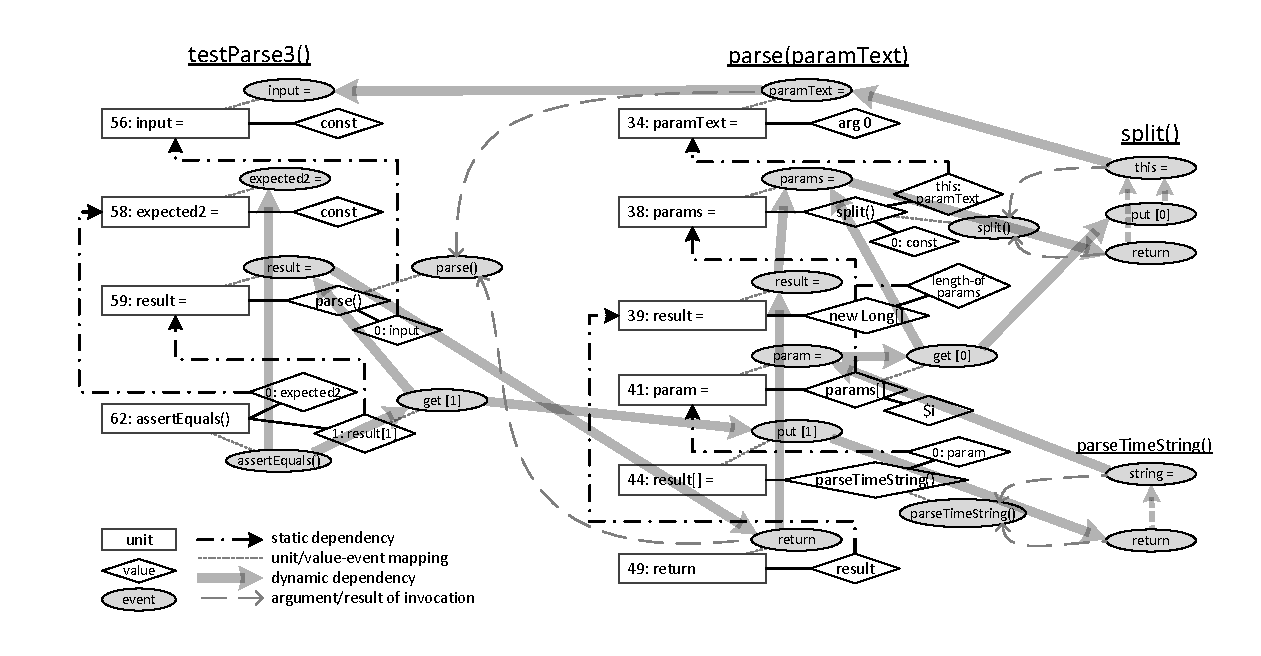
\includegraphics[width=\linewidth, clip, trim=12mm 7mm 8mm 7mm]{img/graph}
%\caption{A dynamic dependency graph of trace events, on top of static dependency graphs derived with Soot. For brevity, not all Soot units are shown, the boxing of long values has been omitted, and ``split'' and ``parseTimeString'' are summarized.}
%\label{fig:graph}
%\end{figure*}

\subsection{Computing the Program Dependence Graph}

Our algorithm for computing the \ac{pdg} distinguishes between three dependency types: data, control, and choice dependencies.
The first two types have been used since the original slicing algorithm by Weiser~\cite{weiser_81_program_slicing}.

Data dependencies represent the data flow in a program and occur whenever the value of an instruction is the result of a previous instruction.
For instance, the value of ´words´ in \linerefn{lst:countLetters}{5} of ´countLetters´ depends on the result of ´split´.

Control dependencies model the control flow and point to instructions that determine whether a statement can be reached during the execution.
The assignment in \linerefn{lst:countLetters}{8}, for instance, has reachability dependency to the conditional expression of the for-loop in \linerefn{lst:parse}{7}.

Choice dependencies occur when a statement has multiple possible data dependencies.
In the statement ´var = foo ? bar : baz´, the value of ´var´ depends on either ´bar´ or ´baz´, but never both.
Even though ´foo´ does not directly affect the value, it determines which of the two options is used; thus, it is a choice dependency.
More formally, choice dependencies are control dependencies of data dependency candidates that are not also control dependencies of all other candidates.
Unlike the other two dependency types, choice dependencies are not simple edges in the graph, but rather tree-like structures.
\Cref{lst:choiceExample} shows an example of a nested choice dependency.
Variable ´x´ in \linerefn{lst:choiceExample}{9} has three value dependency candidates, shown with solid red arrows. 
The choice dependencies, shown as dashed blue arrows, link to the conditional expressions that determine the choice.
The relation between the five dependencies is modeled in the tree structure.

It should be noted that choice dependencies are redundant for the purpose of computing accurate slices, which is why they were never considered in related literature.
However, as we will discuss in more detail in \todo{reference}, including this dependency type allows us to create slices closer to a developer's needs.

\begin{lstlisting}[float,caption={Example of a nested choice dependency.},stepnumber=2,numberfirstline=false,label=lst:choiceExample,language=Java]
  /*@\hspace{7mm}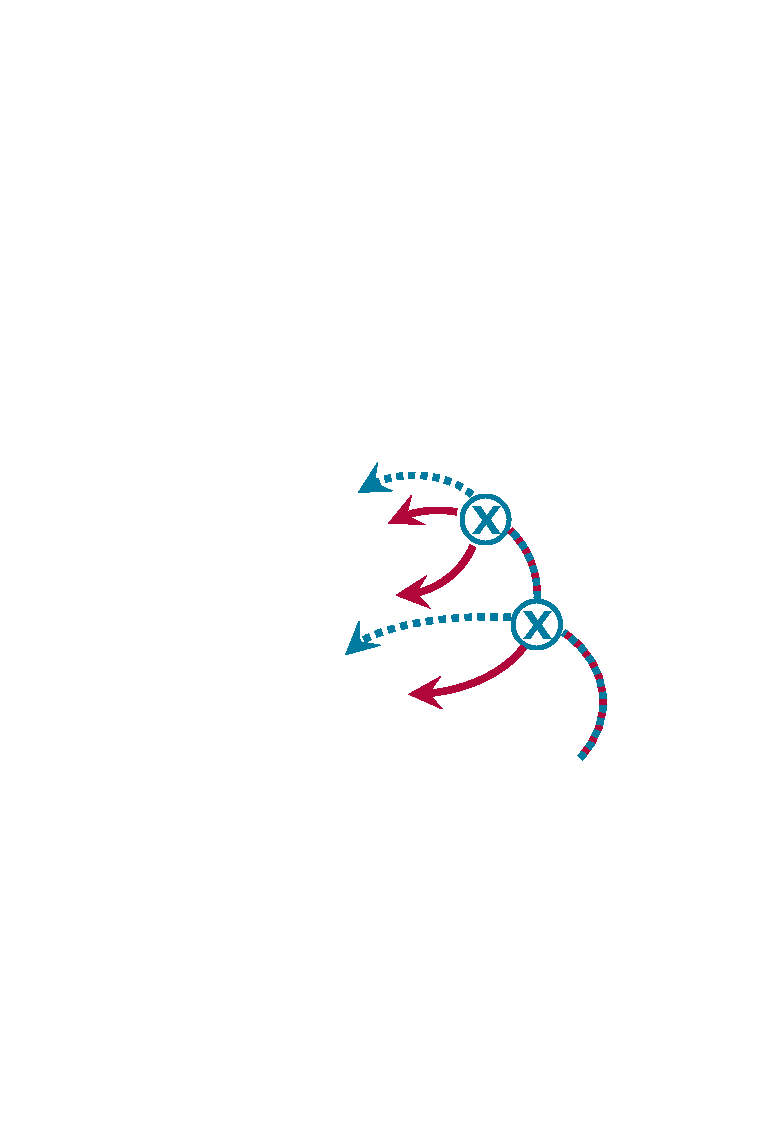
\includegraphics[width=34mm, trim=0mm 45mm 0mm 7mm]{img/choiceexample.pdf}\hspace{-41mm}@*/if (a) {
	  x = 1;
	} else {
	  x = 2;
	} 
	if (b) {
	  x += 2;
	} 
	System.out.println(x);
\end{lstlisting}

The algorithm to build the method-level \ac{pdg} was implemented in Soot, using a \emph{forward flow analysis}~\cite{lam_11_the_soot_framework}.
The analysis algorithm has two major operations, the visit and the merge.

In Soot, a method is represented by three-address-code instructions, called "units".
A flow analysis "flows through" (i.e., visits) every unit in a method and allows to pass state in a "flow set" from one instruction to the next.
In our case, the flow set is the \ac{pdg}, as it was computed so far, plus some additional index structures.
The visit operation consists of two steps, as is outlined in \cref{lst:visit}.
First, it collects the dependencies for referenced values, 
then, it creates a node representing the current instruction and adds it to the \ac{pdg}, accordingly to its type.

%\begin{algorithm}
%\caption{The algorithm of the visit operation.}
%\label{lst:visit}
%\begin{lstlisting}[firstnumber=1,stepnumber=5,gobble=0,language=algorithm,tabsize=2]
\begin{lstlisting}[firstnumber=1,float,caption={The algorithm of the visit operation.},stepnumber=5,label=lst:visit,gobble=0,language=algorithm,tabsize=2]
function visit(pdg, unit)
	result := 'copy of' pdg
	dependencies := dependencies_of_values(unit.use_boxes, result)
	if unit 'is a conditional statement' then
	  d := new ControlDependencyNode(dependencies)
		result.control_dependencies.push(d)
	else
	  d := new DependencyNode(unit, dependencies, result.control_dependencies.peek())
		result.store_dependency(unit, d)
		if unit 'is an assignment' then
			result.index_assignment(unit.left, unit)
			if unit.left 'is a variable' then
				result.set_variable_node(unit.left.name, d)
		else if unit 'is a return statement' then
			result.index_return(unit)
		else if unit 'is a throw statement' then
			result.index_throw(unit)
	return result

function dependencies_of_values(values, pdg)
	dependencies := {}
	for each v \in values do
		dependencies << dependency_of_value(v, pdg)
	return dependencies

function dependency_of_value(value, pdg)
	if value 'is a local variable' then
		return pdg.get_variable_node(value.name)
	else if value 'is a method invocation' then
		d := new MethodInvocationNode(value.method, 
				dependency_of_value(value.instance, out), 
				dependencies_of_values(value.arguments, out))
		pdg.index_invocation(d)
		return d
	else if value 'is a field reference' then
		return new FieldReferenceNode(v.name, dependency_of_value(v.instance))
	else 
		'handle other value types...'
\end{lstlisting}
%\end{algorithm}

For each unit that is visited, its dependencies are determined from its "use boxes", the values accessed by the unit (cf.~\linesrefn{lst:visit}{3, 20-38}).
\tmpStart
To obtain a list of dependencies from a list of value boxes, each value is examined independently.
If it refers to a variable, the node currently associated with that variable is used.
Field and array accesses are not investigated any further, but a placeholder node is created instead.
Method invocations are also treated as opaque, and no dependency between the invocation result and its arguments is created.
Instead, the dependencies for each argument are determined separately and directly added to the index, with a unique key being created for each argument.
It is expected that the subsequent analysis of the invoked method reveals, if necessary, if and how an invocation's result depends on its arguments.
\tmpEnd

If the unit represents a conditional statement, the dependencies are pushed to the control dependency stack.
Otherwise, they are data dependencies of the unit.
If the unit assigns a variable, it is also registered to be the last unit that changed that variable.
Furthermore, each unit is indexed (cf.~\linesrefn{lst:visit}{10-17, 33}).
The index is stored as a map and will be used later to find the units for recorded events.

The result of the visit step is passed as input to the next unit's visit operation.
If a unit has more than one following unit, (e.g., if it is a conditional jump) a copy of the flow set is passed to each.

When control flow merges, e.g., after a conditional branch closes, two or more flow sets have to merge into one, which can then be passed to the next unit.
Thus, the second major operation of our algorithm is the merge. 
In the merge step of the analysis, the result is a copy of the first incoming flow set, which is then merged with the second incoming set, as outlined in \cref{lst:merge}.

\begin{lstlisting}[firstnumber=1,float,caption={The algorithm of the merge operation.},stepnumber=5,label=lst:merge,gobble=0,language=algorithm,tabsize=2]
function merge(in1, in2)
	result := 'copy of' in1
	if in2.control_dependencies != result.control_dependencies then
	  choice_dependencies := 'disjunctive union' in2.control_dependencies \delta result.control_dependencies
		result.control_dependencies.remove(choice_dependencies)
	else
	  choice_dependencies := {result.control_dependency_stack.pop()}
	for each var \in in2.variable_nodes do
		result_value := result.get_variable_node(var.name)
		if var.value != result_value then
      merged_value := new ChoiceDependencyNode(
            choice_dependencies, var.value, result_value)
			result.set_variable_node(var.name, merged_value)
	return result
\end{lstlisting}

To merge two flow sets, first their control dependency stacks have to be aligned.
If the stacks contain different elements, only dependencies from both stacks are kept.
If both stacks are identical, for instance when merging the then- and else-branch of an if-statement, the topmost element of the stack is removed.

Then, all variables that have different values have to be merged.
Instead of a definite unit, the new value is a choice of the two previous values, indicating that in the dynamic slice only one of the options will actually apply.
Thus, the control dependencies that have been removed during the merge are added here as choice dependencies.

By visiting all instructions in a method and merging the intermediate \acp{pdg} of all possible execution paths, the algorithm eventually produces a complete method-level \ac{pdg}.
For reference, \cref{fig:graphstatic} shows the data dependencies of the \acp{pdg} of ´countLetters´ and ´testCountLetters´.

\begin{figure*}[t]
\centering
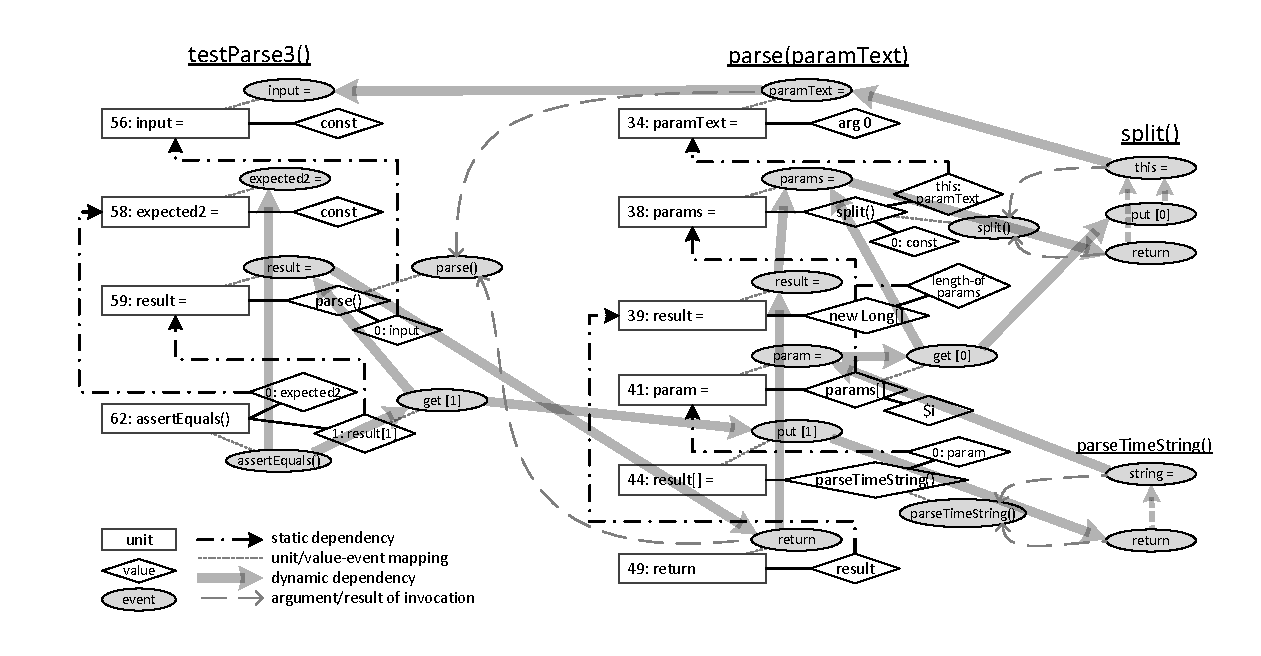
\includegraphics[width=.90\linewidth, clip, trim=12mm 7mm 8mm 7mm]{img/graph}
\caption{The method-level \aclp{pdg} of \lstinline+countLetters+ and \lstinline+testCountLetters+.}
\label{fig:graphstatic}
\end{figure*}

\subsection{Mapping Events and Units}



%Previous "accurate" dynamic slicing algorithms based on \acp{ddg} work by first building a complete \ac{ddg} and then deriving the slice as a subgraph~\cite{agrawal_90_dynamic_program_slicing,zhang_03_precise_dynamic_slicing_algorithms, wang_08_dynamic_slicing_on_java}.
%Our algorithm builds the \ac{ddg} and the slice together, constructing only as much of the \ac{ddg} as is needed to compute the slice.
%Since the method-level \acp{pdg} that form the foundation for the \ac{ddg} are also computed on demand only, our algorithm can potentially save a lot of unnecessary work.

The \ac{ddg} is built by combining the \acp{pdg} with an execution trace.
In the \ac{ddg}, every node is an event, a recorded execution of an instruction.
However, for the purpose of slicing, we consider only events that have a side-effect on the program state, i.e., variable or field assignments, or cause non-local control flow, such as method calls and returns.


The basic structure of the algorithm for building the initial slice is summarized in \cref{lst:slicealgo}.

\begin{lstlisting}[float=t,language=algorithm,label=lst:slicealgo,caption={Simplified algorithm for building the slice}]
	function build_slice(criteria)
		slice := {}
		for each event \in criteria do
			''asynchronous:'' add_to_slice(slice, event)
		return slice
		
	function add_to_slice(slice, event)
	  if ~event.has_unresolved_dependencies then return
		slice << event
		pdg := event.method.program_dependence_graph
		static_dependencies := pdg.get(event.instruction, event.dependency_flags)
		for each dependency_link \in static_dependencies do
			for each prev_event \in last_previous_events(event, dependency_link) do
			  prev_event.inherit_dependency_flags(event)
				''asynchronous:'' add_to_slice(slice, prev_event)
\end{lstlisting}


Before the dependencies of an event can be found, it has to be mapped to a Soot unit.
The event provides class and method name, line number, and byte-code index as locational information.

Alas, we were not able to find the corresponding unit based on the byte-code index.
Instead, the event type and line number are used to look-up units in the index that was created during the flow analysis.
For an averagely structured Java program, ambiguities occur only rarely.
As shown on the bottom left of \autoref{fig:graph}, in our example the slice would begin with the \verb+assertEquals+ invocation, which can be mapped to the invocation unit in \linerefn{lst:test}{62}.

Once the unit has been identified, its dependencies are looked-up and converted back to events.
Reachability dependencies are included only if they have been explicitly requested.
%How events are looked-up depends on the type of the dependencies.
The dependency value's line number and the current event's step number are used to identify the most recent matching event.
However, the strategy of the look-up also depends on the type of the dependency value.

If the dependency is an assignment statement of a variable, the last variable change event in that line is looked-up.
For instance, the dependency between the \verb+assertEquals+ invocation and the \verb+expected2+ assignment is created this way.
If it is a choice of multiple variable assignments, each assignment is looked-up and, if more than one is found, only the most recent will be used.

For field and array value dependencies, first the according get-event is looked-up.
Then, the last set-event before the get is found.
For instance, this allows us to create a dynamic dependency between \verb+assertEquals+ and the array assignment in the second iteration of \verb+parse+ (shown on the right-hand side of \autoref{fig:graph} as the ``put'' event linked to the assignment in \linerefn{lst:parse}{44}).
Finding the get as an intermediate step is necessary to avoid situations where the field has been changed between access and usage, e.g., as in \verb/int id = counter++/.

If the value stems from an argument, first the calling method is determined from the trace data. 
Then, the argument is looked up in the index of the dependency graph of the calling method.
Finally, the dependencies retrieved this way are resolved recursively.
To get the result of an invocation, the method call event is looked-up and its respective return event is found.
As \autoref{fig:graph} shows, the invocation of \verb+parse+ is not part of the dynamic dependency graph because it is an event without side effects.
However, it serves as the link to create dependencies between events of the two methods.

All events that are found this way are added to the slice.
If an event was found via a unit, this information is retained and reused when computing the dependencies for that event.

The final list of events is the used by the debugger to visualize the program flow and to skip unrelated events during stepping.

In principle, the Slice Navigator can run on top of any slicing algorithm.
However, for most effectiveness, the algorithm should satisfy three criteria:
First, it should be able to quickly produce useful intermediate results to avoid interrupting developers in their work.
Second, if it distinguishes between different types of dependencies, the differences between those types should be easily understandable for developers.
This way, additional helpful information can be communicated to the user and better customization of the slice is possible.
Finally, it should support incrementally changing the slicing criteria.
The algorithm we use in our prototype is specifically engineered to meet these criteria.

%The algorithm we use in our prototype is based on previous work~\cite{treffer_dynamic_2014} and specifically engineered to meet these criteria.
%When building the dependency graph between instructions, the algorithm distinguishes between three types of dependencies.
%
%\emph{Value dependencies} occur when the the value of an instruction is derived from another instruction's value.
%In the slice navigator, they are represented with a red equality sign.
%
%Instructions that determine if another instruction can be reached are \emph{reachability dependencies}, indicated by a yellow arrow.
%Typically, these are method invocations and instruction in conditional statements.
%
%Sometimes, a value depends on only one of multiple candidate values. 
%A \emph{control dependency} determines which of these candidates is used.
%More formally, control dependencies are reachability dependencies of value candidates that are not also reachability dependencies of all other candidates.
%In the navigator, they are indicated by a blue~"X".
%
%Developers can now combine these different dependency types to adjust the slice for specific purposes.
%Clicking on an event's dependency symbol brings up a dialog that allows to choose which dependencies of that event to include.
%This way developers can, for instance, put a focus on how a value was computed or how an instruction was reached.
%It is also possible to remove all dependencies of an event, for instance if it is known to be correct and its history is not of interest, thereby moving the focus of the slice to less well-understood parts of the program.


Typically, static and dynamic slicing algorithms focus on finding statements belonging to a slice.
However, in many cases statements are executed multiple times in a single program run and not all executions are relevant for the slice.
Therefore, our algorithm focuses on state-changing events, i.e., actual executions of statements, instead of the statements themselves.

On the highest level, our algorithm to compute a dynamic slice works as follows:
The output of the algorithm will be a sorted set of events.
The target event, i.e., the event for which the slice was requested, is added to both the result set and a queue of unprocessed events.
Then, until the queue is empty, an event is polled and its dependency events are determined as follows:

%Firstly, the event is mapped to a unit of a \verb+SootMethod+.
Firstly, the event is mapped to a statement in the code.
Secondly, Soot is used to obtain a static dependency graph for that method (the graph is cached for reuse).
Thirdly, the statement is looked-up in the graph and candidate dependency statements are mapped back to events.

Each dependency event that is not yet part of the result set is added to both the result and the queue.
Finally, the result set is returned.

\begin{figure*}[t]
\centering
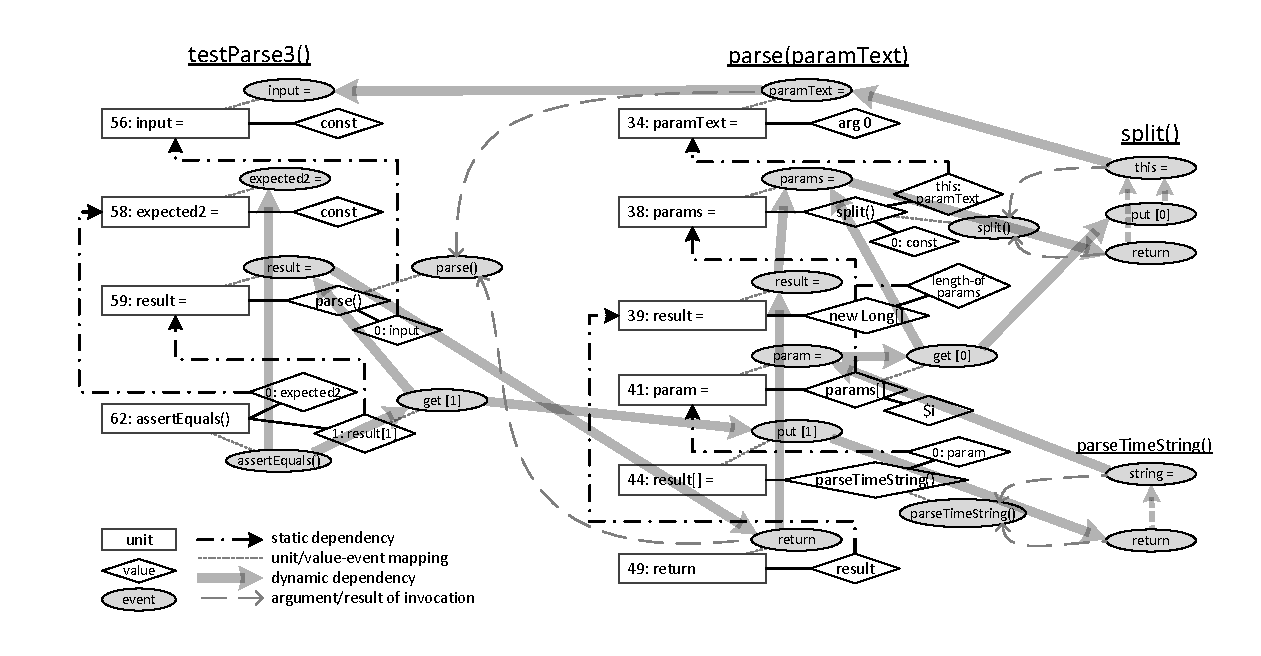
\includegraphics[width=.90\linewidth, clip, trim=12mm 7mm 8mm 7mm]{img/graph}
\caption{A dynamic dependency graph of trace events, on top of static dependency graphs derived with Soot. For brevity, not all Soot units are shown, the boxing of long values has been omitted, and ``split'' and ``parseTimeString'' are summarized.}
\label{fig:graph}
\end{figure*}
\tmpEnd

\tmpStart

\section{A New Debugging Workflow}
\label{sec:workflow}

Both omniscient debugging and (dynamic) slicing changed the way how developers approach fault localization.
In this section, we use a simple example to demonstrate how we integrated existing and new tools to an improved debugging workflow.
We also describe the user interface of the Slice Navigator, how it presents information about the slice, and how it can be used to control the debugger.

\subsection{Getting Started}
\label{lst:example}

Very often, the starting point for a debug session is a reproducible observable program failure, preferably in the form of a failing unit test.
Using an omniscient debugger, developers halt the execution at the failing line of code to observe the program state.
From here, they want to backtrack the erroneous state.
However, they quickly realize that the code contains many other side effects making it hard to follow the state of interest.

Using a pure omniscient debugger, developers would now have to track the relation of states to identify the infection chain. 
In other words, they have to manually create a dynamic dependency graph using only their short-term memory. 
When slicing features are supported, they might rather leave that task to the tools.

For instance, using our tool, developers can right-click the erroneous state in the debugger's variables view and choose slicing from the context menu.
This will set the variable or field as a slicing criterion and start the slice computation.

%The initial code analysis can take a few seconds.
%The performance of our prototype implementation is evaluated in \todo{section ?} .
Once the slice is computed, all debugging views (e.g., the trace and the variable view) will show instructions or variables not belonging to the slice only in gray.
Stepping through the execution will skip instructions not belonging to the slice.

We will use a small code example to explain the user interface and internals of the Slice Navigator. 
\Cref{lst:example} shows two Java classes and a failing JUnit test case.
In our scenario, after noticing a failed test case, the developer chooses to slice on the arguments of the ´assertEquals´ invocation in \linerefn{lst:example}{31}.
Because we are using only a minimal example, the resulting slice contains almost the entire program.
When we tested the Slice Navigator on real open source programs, this step often already removed a lot of code.

Nevertheless, for a complex program the initial slice can still be too large to allow an efficient search for the problem.
In this case, the developer can now use the Slice Navigator to get an overview of the execution and to iteratively adjust the slicing criteria.

\begin{lstlisting}[float=t,label=lst:example,caption={Example program with a failing test case}]
	class Square implements Shape2D {
		private double length;
		public Square(double length) { 
		  this.length = length;
		}
		
		@Override
		public double getArea() { 
			return length * length;
		}
	}
	
	class Pyramid implements Shape3D {
		private Shape2D base;
		private double height;
		public Pyramid(Shape2D baseShape, double height) {
			base = baseShape;
			height = height;
		}
		
		@Override
		public double getVolume() { 
			return base.getArea() * height / 3; 
		}
	}
	
	class PyramidTest {
		@Test
		public void test_getVolume() {
			Shape3D shape = new Pyramid(new Square(2), 6);
			assertEquals(8, shape.getVolume());
		}
	}
\end{lstlisting}

\subsection{The Slice Navigator}

\begin{figure}
  % picture on first page :)
	\centering
		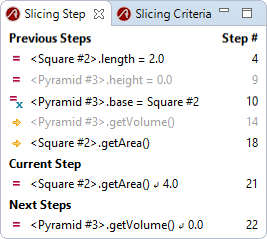
\includegraphics[width=0.40\linewidth]{img/slice1.png}
	\caption{The Slice Navigator shows context for the current debug step. Steps directly related to the current step are listed in black, steps with overarching dependencies in gray. Small icons indicate how the steps are related.}
	\label{fig:slice1}
\end{figure}

To produce a slice, dynamic or static, slicing tools have to build up deep knowledge of a program's internal workings.
In the end, only a binary mapping about which instruction to include or exclude from the program is returned, and most of the slicer's internal knowledge is discarded.
Hence, the initial motivation for the Slice Navigator was to make better use of a slicer's internal data.
However, since the size of all dependency graphs is typically too vast to be visualized at once, we propose to use that data to guide developers while they debug the slice.

The first purpose of the Slice Navigator is to aid the developer's short-term memory.
It provides a quick overview over previous and upcoming events, and how they relate to the current instruction.
\Cref{fig:slice1} shows a screenshot of the slice navigator with the execution of the example test-case halted on the ´return´ instruction of ´getArea()´ in \linerefn{lst:example}{7}.

A step, or event, is any instruction that has a side effect on the program state.
"Previous Steps" lists all past events that the current or any future events depend on.
Likewise, "Next Steps" shows all events that depend on the current or a previous event.

If a step is shown in black, it has a direct dependency link to the current step.
Steps shown in gray have dependencies that go beyond the current step.
I.e., gray "previous steps" have dependency links to "next steps", and vice versa.

Simply by looking at the previous and next steps, the developer can understand at a glace how the current instruction fits into the greater scheme.
This is particularly useful if the current instruction was reached via a breakpoint, in which case it is not always obvious at which point in time it was hit.

To obtain this kind of information with a regular debugger, developers need to analyze the execution stack and maybe even inspect lower stack frames.
But even then it is not always obvious which part of the program state that is still reachable is actually used again.
Unlike a typical debugger's variable view, the Slice Navigator only shows relevant variables, and also shows relevant object fields on the first level.

Further, the Slice Navigator shows details about the dependency graph that was used to compute the current slice.
Small icons indicate how the events of the slice are related.
The meaning of these symbols will be explained in the next subsection.

The second purpose is to serve as a convenient interface to the debugger.
Debugging with the Slice Navigator is simple:
To investigate the origin of a value, developers can simply click on it to move the execution to that point in time.
This way, the slice navigator allows to efficiently follow infection chains of erroneous state.
Likewise, it is easy to follow up on the impact of an instruction by navigating to its future dependencies.

However, using the Slice Navigator developers can not only control the debugger, they can also adjust the slicing criteria.



\section{The Slice Navigator}

\section{Performance Considerations}
\label{sec:eval}

\section{User Study}

\tmpStart
We evaluated our approach in two ways.
First, we measured the run-time of the slicing component for various operations on a real-world project and found it to be fast enough to be usable in practice.
Second, we let developers locate bugs using different tools and interviewed them about their experience.
The experiment confirmed the usefulness of the Slice Navigator and provided suggestions for further improvements of our tool.

\subsection{Performance Considerations}

One of the main advantages of the Slice Navigator is that it integrates into the debugging workflow.
As such, it is crucial that results are produced in a timely manner, as a waiting time of even a few seconds may interrupt developers in their flow.

To evaluate the performance of our approach on real-world code, we measured the computation of several slices on JUnit tests of an open-source business-process engine\footnote{\url{https://github.com/camunda/camunda-bpm-platform}}.
All tests were run on a 2.0 GHz Intel i7 Processor with 4 cores and and 8 GB RAM, running Windows 8.1.
A MySql database was used to store the trace data.
We repeated every measurement 10 times, all charts show the average values.

\begin{figure}
	\centering
		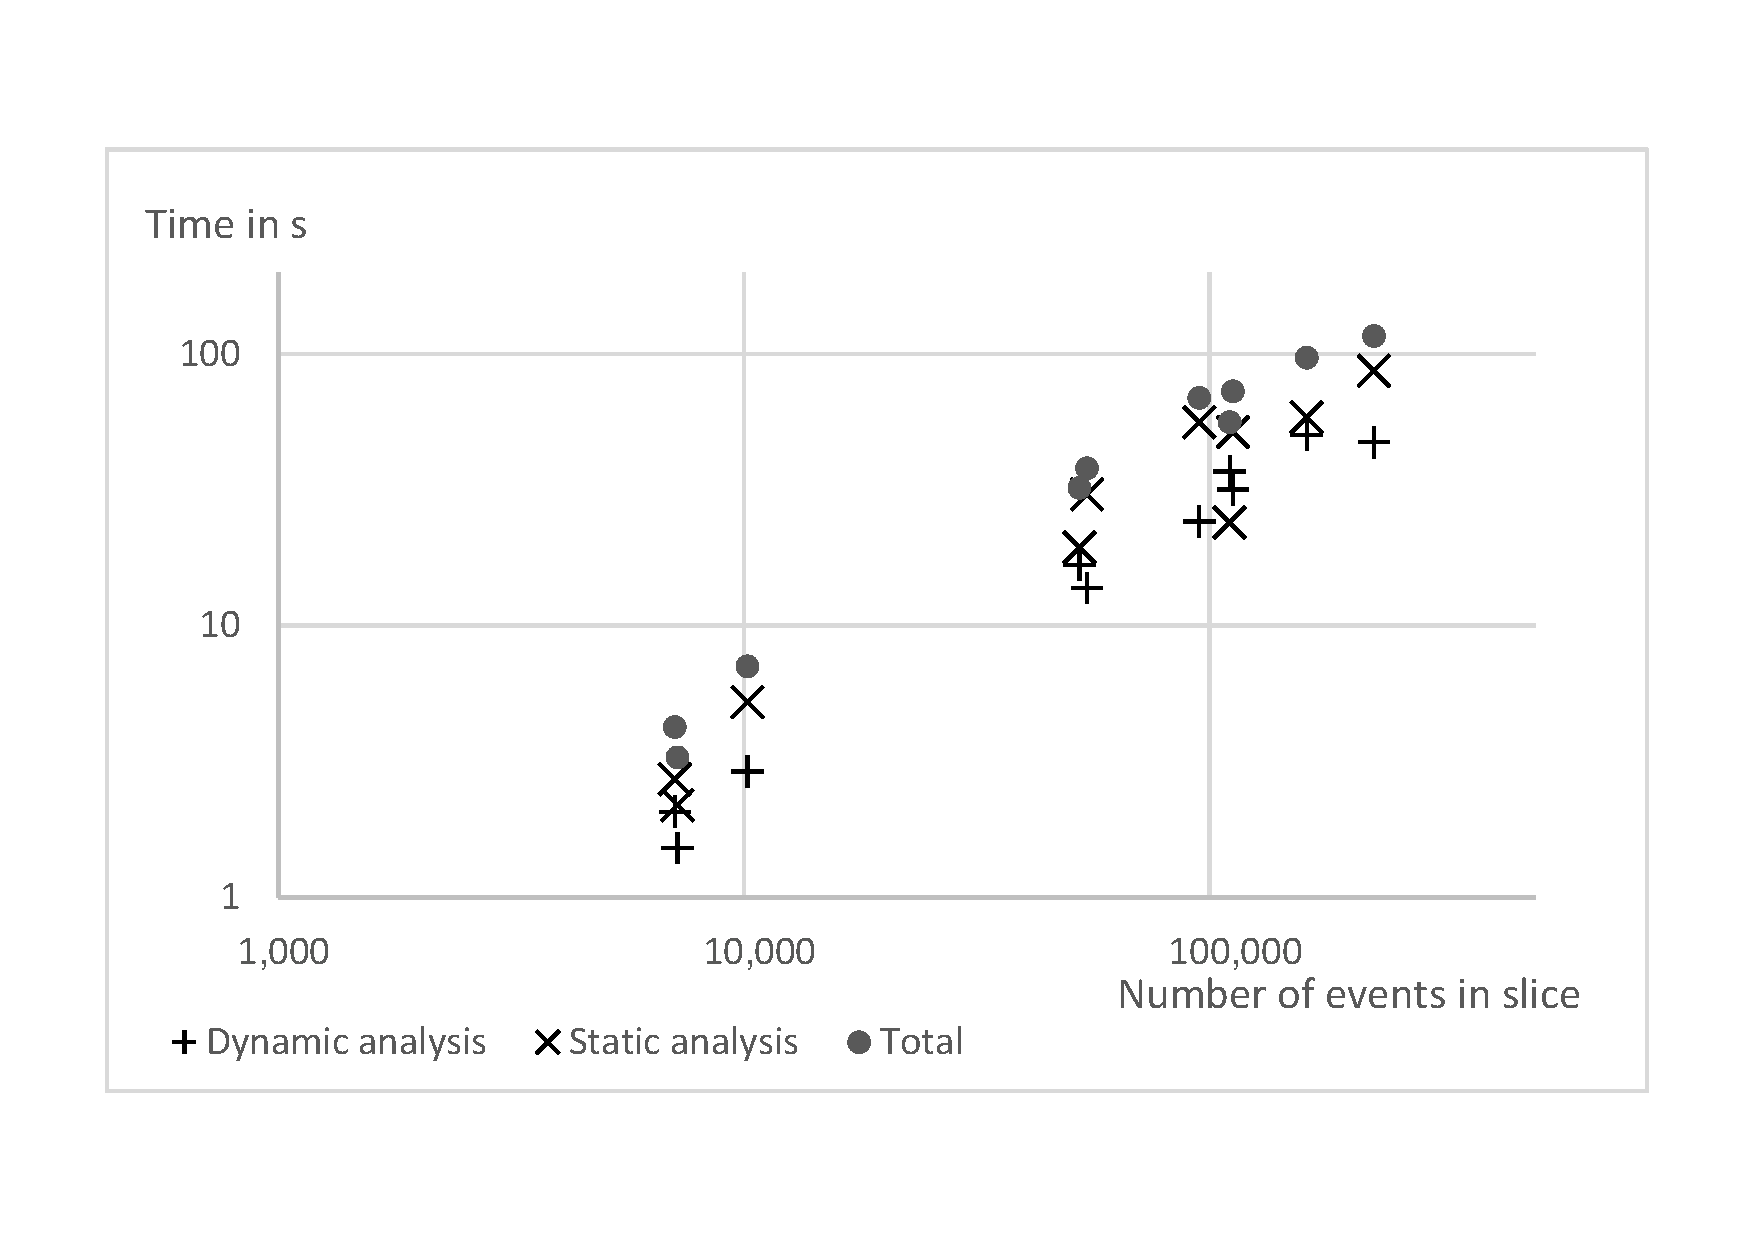
\includegraphics[width=\linewidth, clip, trim={20mm 26mm 20mm 26mm}]{img/chart-initial.pdf}
	\caption{Time for computing the initial slice}
	\label{fig:chartinitial}
\end{figure}

We previously observed that our approach differs from other slicing implementations insofar as that the run-time of the algorithm does not depend on the total length or run-time of the sliced program, but only on the size of the resulting slice~\cite{treffer_dynamic_2014}.
Our current measurements confirm that slicing time is linear to the result size.

\Cref{fig:chartinitial} shows the time for computing the initial slice in seconds, depending on size of the resulting slice.
Times are given in total, and divided into static code analysis and the dynamic analysis of the event data.

As can be seen, the static analysis takes slightly more time on average.
It should be noted that the total time is less than the sum of the static and dynamic analysis times, as both can, to some extent, run in parallel.
The chart shows that in our setup the algorithm was able to process approximately 1000 events per second.

\begin{figure}
	\centering
		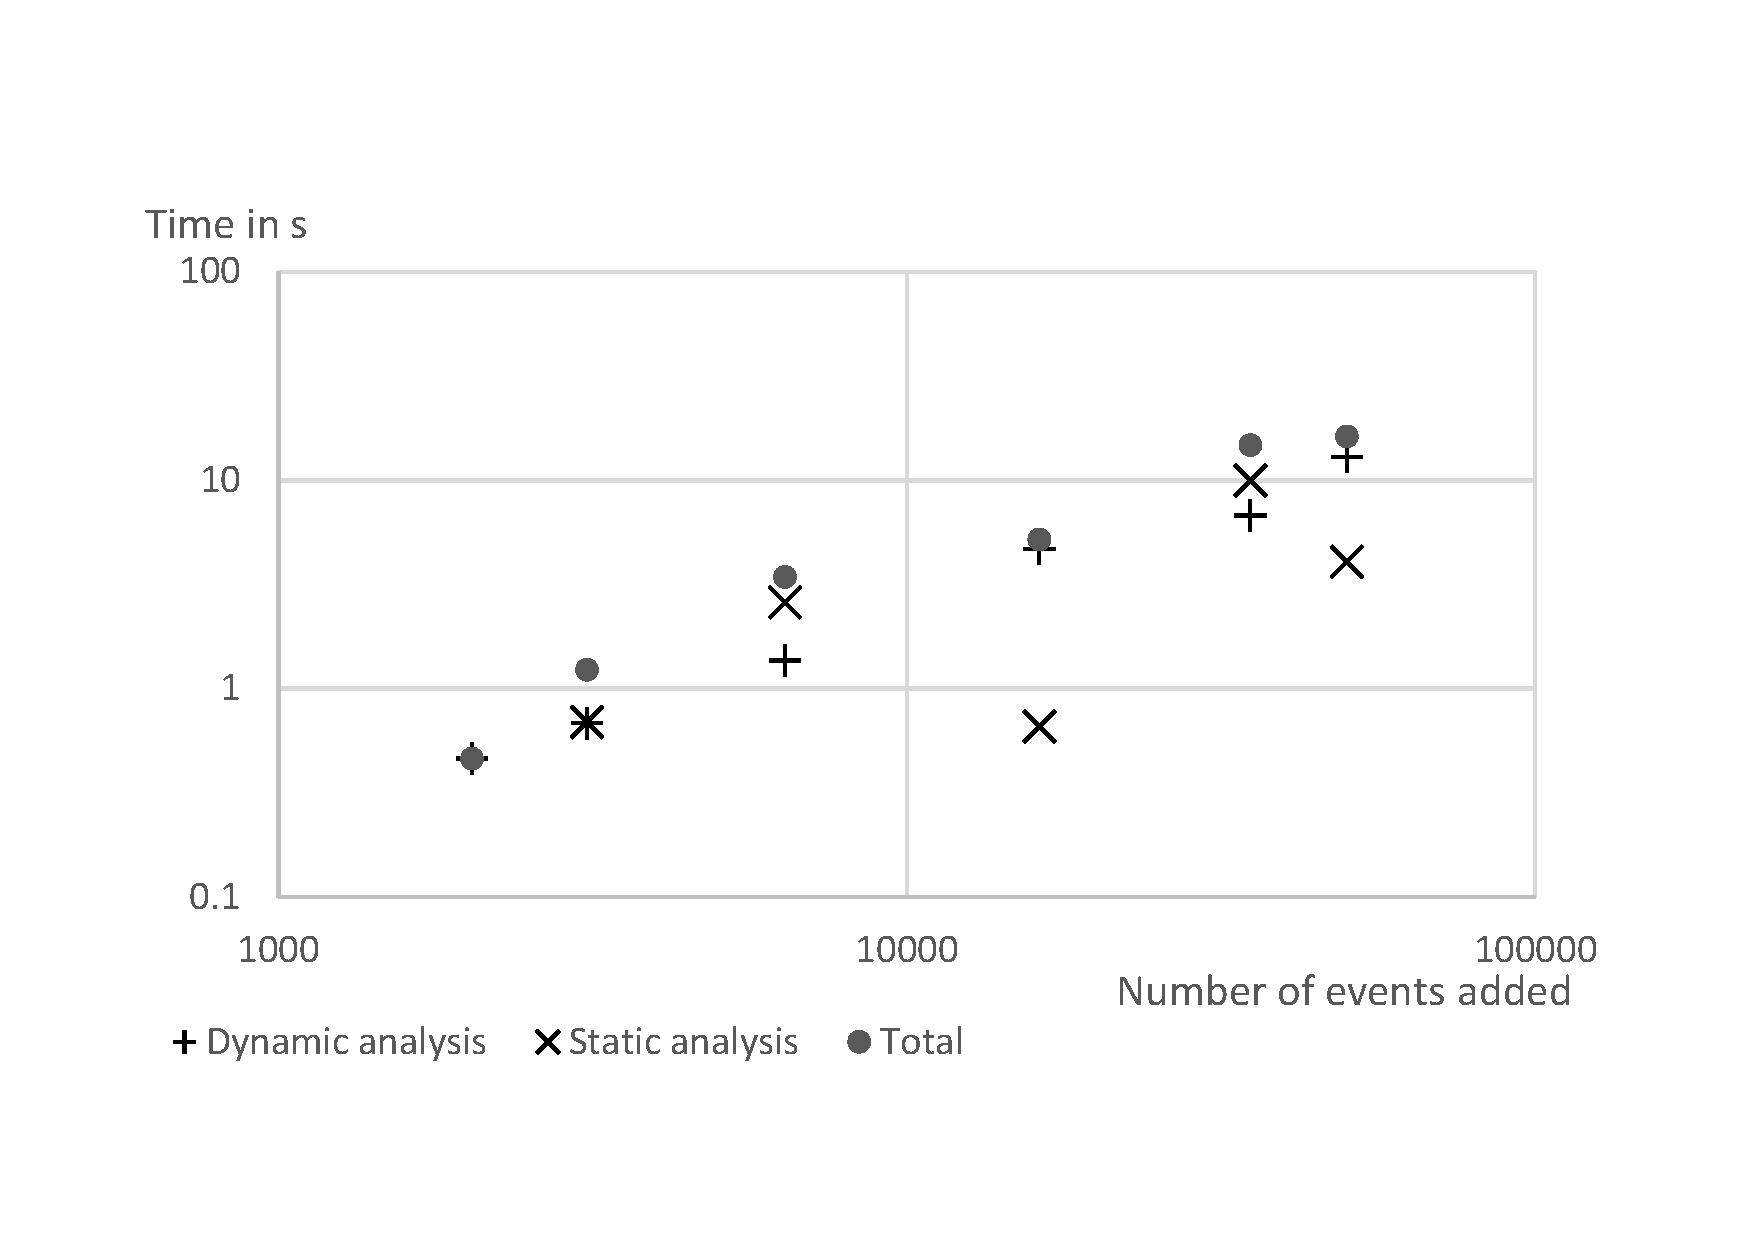
\includegraphics[width=\linewidth, clip, trim={20mm 26mm 20mm 26mm}]{img/chart-add.pdf}
	\caption{Time for adding a slicing criterion}
	\label{fig:chartadd}
\end{figure}

When adding additional elements to the slice, previously computed dependency graphs can be reused.
As \cref{fig:chartadd} shows, the time for dynamic analysis remains constant per event.
The time for static analysis, on the other hand, shows great variation and depends on how much new code was included by the broadened slicing criteria.
In the worst case, expanding the slice takes as long as creating a new slice for only that event.

\begin{figure}
	\centering
		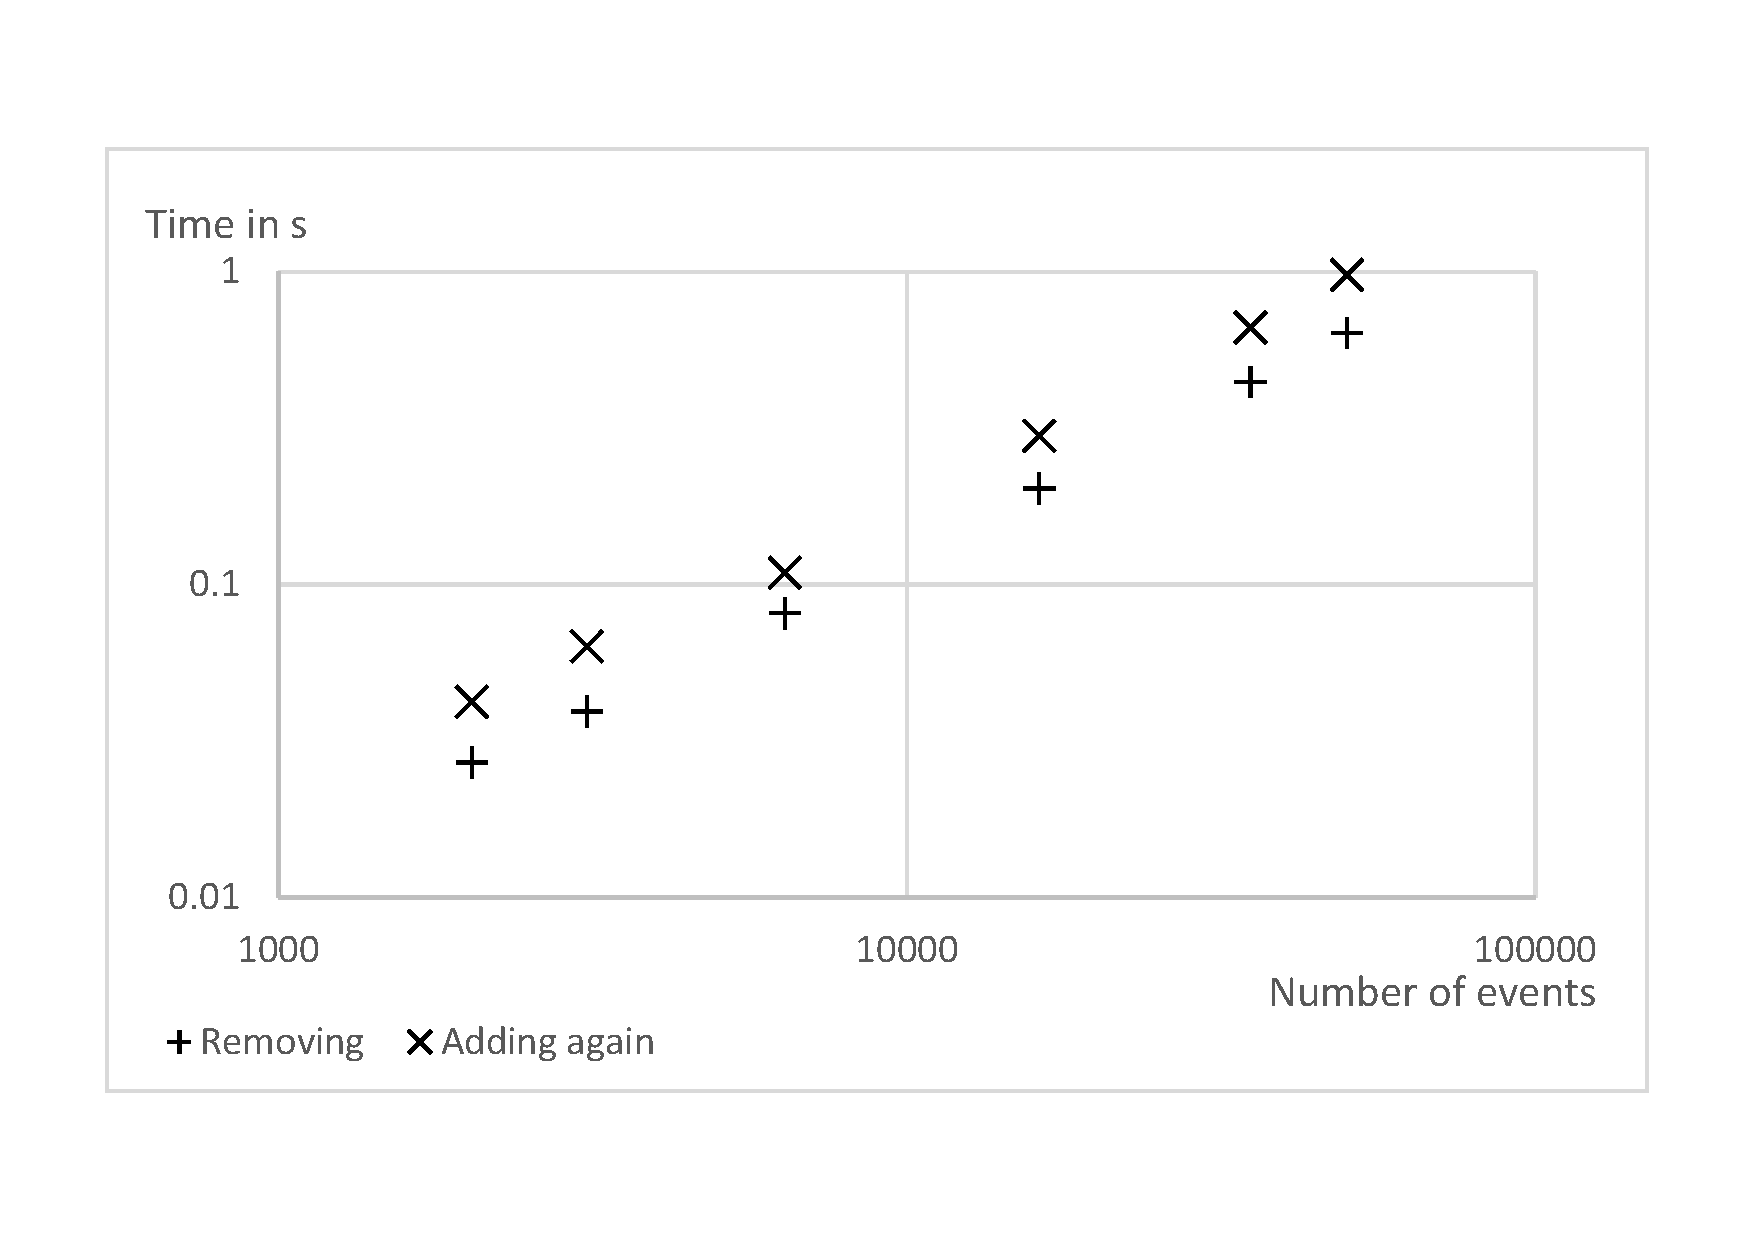
\includegraphics[width=\linewidth, clip, trim={20mm 26mm 20mm 26mm}]{img/chart-rem.pdf}
	\caption{Time for removing events from the slice}
	\label{fig:chartrem}
\end{figure}

\Cref{fig:chartrem} shows that removing events from the slice by narrowing the slicing criteria is significantly faster, as no actual analysis has to be performed.
Likewise, adding those events again by reverting the slicing criteria change is fast, as previously computed dependency graphs can be reused.

\medskip

From the results in \cref{fig:chartinitial}, it seems as if the slicing algorithm is too slow to be of practical use to a developer.
A single second of execution can produce several hundreds of thousands of events and it is generally not feasible to wait multiple minutes for the slicing to complete.
However, due to parallelization and the way the algorithm works, developers experience a delay of only a few seconds.

As described above, the debugging user interface is updated with an intermediate slicing result twice per second.
The slicing algorithm works its way backwards, beginning at the slicing criteria.
Then, previous events are processed not ordered by their absolute position in the execution, but by their distance in the dependency graph.
As a result, both the near past and long-running overarching method invocations are processed first.

This allows developers to begin debugging the slice almost immediately. 
From this point on, the slicer only needs to be faster than the developer moving backwards, which is generally given.

For interactive changes of slicing criteria, our experiments have shown that the incremental slicing algorithm is fast enough to not interrupt the developers flow.
In particular, the most common operation -- removing events by narrowing the slicing criteria -- completes in less than a second even for large numbers of events.
From this we conclude that our debugging approach, based on the Slice Navigator and on iterative slice refinements, is generally feasible.

\subsection{User Study}

To gather empirical data on the usefulness of our approach, we conducted an experiment where we let developers locate bugs using a regular debugger, the omniscient debugger from our debugging framework, and the Slice Navigator, and compared their experiences.

We used Defects4J, a database of actual bugs from various open-source projects~\cite{just_defects4j_2014}, to find suitable debugging tasks.
For each bug, Defects4J also provides at least one failing test case and the fix.

We chose to conduct the experiment with \emph{Joda Time}\footnote{\url{http://www.joda.org/joda-time/}}, a date and time library for Java, because it has a domain that everyone is already familiar with.
From the Defects4J bug database, we selected Joda Time bugs 10, 19, and 27.

The bugs were selected because they can be fixed with a small change at a single code location and require not much knowledge about the more technical details of Joda Time.
Furthermore, all bugs are from different parts of the project, so that in our experiment the order of the bugs will have no impact on the developers' familiarity with the code.
Finally, each bug is caused by a different kind of defect:
the first bug is caused by a wrong hard-coded constant value;
the second bug is caused by wrongly skipped code, i.e., a too restrictive \textit{if}-condition;
while the third bug is caused by code that should be skipped, i.e., a missing \textit{if} statement.
We expect that the usefulness of each debugging tool varies depending on the nature of the bug.

We recruited nine participants for our experiment:
two full-time software developers with at least 15 years of programming experience, 
four PhD students in computer science with at least 10 years of programming experience,
and three computer science graduate students with at least 5 years of programming experience who also worked as programmers in a part-time job for at least one year.
Ages of participants ranged between 25 and 36; one PhD student was female, all other participants were male.
No participant had previous experience with Joda Time, although 5 participants were aware of its existence.

Every participant was tasked to find the location of each bug by debugging the failing test case with one of the tools.
With the Slice Navigator, we specifically asked the participants not to use the other features of the omniscient debugger and reminded them during the task if necessary.
In the end, every participant had used each tool and every bug was examined with each tool three times.

For each debugging task, the procedure was as follows:
First, the participant was shown a passing test case similar to the test case they would later have to debug.
We explained the purpose of the test and started the debugging tool to be used.
Then, we let the participant debug the test case, while we explained both the code and the tool.
When the participant had no more questions, we presented the failing test case and explained the semantics of the failure.
Then we asked the participant to locate the bug using the respective tool and started the timer.
During the debug session, we provided tool support when needed.
If a bug could not be located within 20 minutes, we aborted the task to advance the experiment.

\subsubsection{Comparison of Tool Usage}

\begin{figure}
	\centering
		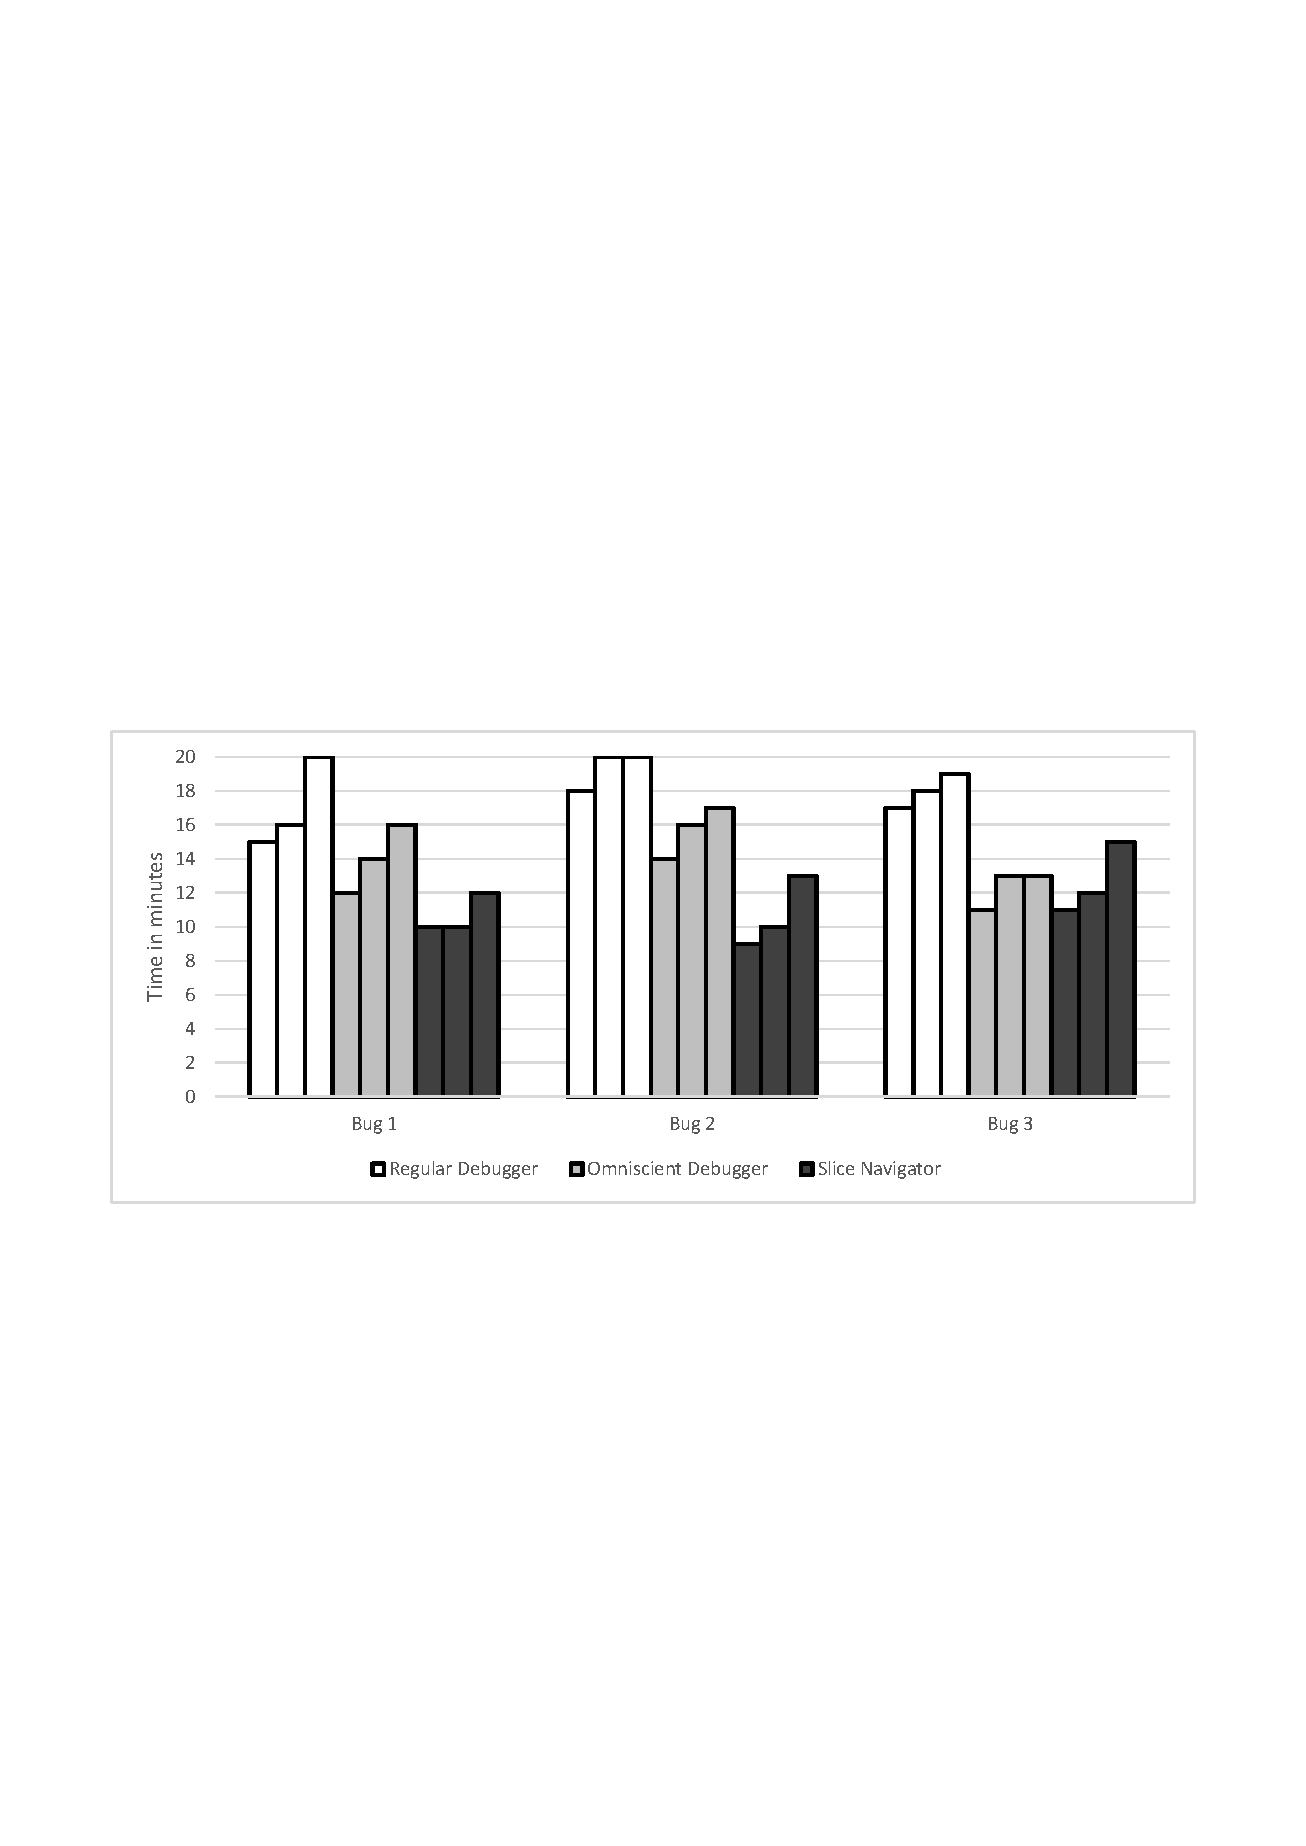
\includegraphics[width=\linewidth, clip, trim={20mm 110mm 19mm 125mm}]{img/chart-times.pdf}
	\caption{Time for solving each debugging task.}
	\label{fig:charttimes}
\end{figure}

\Cref{fig:charttimes} shows the time taken for each debugging task.
The data suggests that the Slice Navigator can make debugging more efficient in many cases.
Furthermore, we observed changes in developer behavior when using different tools.

With the Eclipse debugger, three participants made heavy use of the "inspect" feature, which evaluates any expression from the source without further executing the program.
In particular, when contemplating whether to step into or over a method invocation, these participants used "inspect" to preview the invocation result.
This shows a general need for moving more freely in time.
The three participants who used "inspect" had to restart the debugger 2, 3, and 4 times, respectively, while the other participants restarted between 6 and 12 times, and accidentally stepped over a method between 2 and 5 times per task.

Furthermore, 5 participants stopped using the debugger entirely for more than a minute, and spent 2 to 7 minutes with pure code reading and mentally simulating the program.

The omniscient debugger was particularly effective for the third bug, where all three participants found that a valid field value was overridden by inspecting the object history.
This allowed them to form a good theory about the nature of the bug very early.
However, the method containing the bug was invoked at two different points in time and each time also called itself recursively.
The bug occurred only in one of the four executions.
With the omniscient debugger, it took developers a while to notice and distinguish the different invocations as they jumped through time.
Overall, with the omniscient debugger all 9 developers felt \emph{lost in time} between 2 and 9 times (average 5.4($\pm1.3$)) per debug session.

Finally, while all developers used the omniscient debugger to step back and forth repeatedly to understand the side effects of a piece of code, 7 developers spend most of their time following the infection chain backwards, while 2 developers mostly debugged forwards in time, like they would with a regular debugger.

With the Slice Navigator, all developers followed the infection chain backwards.
Compared to using only the omniscient debugger, developers where able to reach the end of the infection chain faster, felt lost in time similarly often (on average 5.4($\pm2.0$) times), but took longer to recover from being lost as they had spent less time understanding the code.
However, with the Slice Navigator, developers spent only 0.9($\pm0.6$) minutes per task reading code entirely unrelated to the bug, compared to 4.3($\pm1.8$) minutes with the other tools.

\subsubsection{Developer Experiences}

After the experiments, we asked the participants how they experienced working with the different tools.

All participants reported that they found it very helpful to be able to go back and forth in time with the omniscient debugger and felt that they could use it more effectively with more experience, as being used to regular debuggers limited their way of thinking.
7 participants said they were at times overwhelmed with the amount of available options and would probably use more of the more advanced features with more experience.
Furthermore, 6 participants expected they would end up lost-in-time less often with code that they are more familiar with.

For the Slice Navigator, we received similar feedback about moving freely trough time.
Furthermore, all participants liked how the Slice Navigator helped to identify relevant program state.
5 participants perceived this as an improvement in particular to the omniscient debugger, as it was less overwhelming.

However, 4 participants found the overarching dependencies shown in gray to be unnecessary and distracting and emphasized the usefulness of being able to double-click an entry to improve the focus of the slice.
On the other hand, 2 participants said they generally liked the idea of seeing relevant state and would probably find it more useful with code they were more familiar with.

Every participant wrongly clicked or double-clicked an entry at least once and was then unable to recover quickly from the mistake.
Thus, an undo-button was requested by all participants.

Finally, 3 participants reported that while the information provided by the Slice Navigator was very useful, they found it distracted from the actual code.
They liked that with a regular debugger they would rarely have to look away from the code and wished for the slicing context to be visualized within the IDE's code editor.

\subsubsection{Threats to Validity}

The main concern to our study is the small number of participants, which does not allow to generalize the results.
All results could be the product of statistical anomalies.
Furthermore, our participant group was very heterogeneous with respect to programming experience,
although we observed no difference in tool usage or skill level between the different groups.
This effect has been observed in previous studies~\cite{host_using_2000, salman_are_2015}.
Nevertheless, some limitations apply~\cite{mcmeekin_significance_2009}.

Likewise, we only considered three bugs from one library.
Although they are real bugs, they all could be tracked down to one location.
For more complex bugs, or bugs in different types of applications, such as web applications, the usefulness of each tool can differ.
A follow-up study should observe programmers using the tools in practice.

Furthermore, all participants were unfamiliar with the code they had to work with.
We accounted for this in two ways.
First, to achieve the same level of initial knowledge for each task, all bugs were chosen from different parts of the library.
Second, each participant received an introduction to the code to be debugged.
Nevertheless, many participants argued they would have used the tools differently with familiar code.

\tmpEnd